\documentclass[letterpaper,twocolumn]{article}

\usepackage{graphicx}
\usepackage[top=1in, bottom=1in, left=1in, right=1in]{geometry}
\usepackage[dvips]{hyperref}
\usepackage{amsmath}

\author{Luke Fraser}
\title{Programming Assignment 2: \\ Vector Summing}
\date{02/05/15}

\begin{document}
\maketitle
\begin{abstract}
  In this programming assignment we implement a parallel prefix summation of a vector array. The purpose being to show that even inherently serial processes can be parallelized by taking advantage of the associative property of some operations. This property is what makes it useful to perform prefix summation on the GPU. The report will show that for large arrays the use of the GPU drastically outperforms the CPU.
\end{abstract}

\section{Introduction}
Prefix summation is an important aspect of parallel programming. This property is used to parallelize algorithms that would otherwise seem bound to a sequential approach. The use of the associative property is what allows this parallelization to occur. 
\begin{equation}
\begin{split}
  1+2+3+4+5+6 \\ 
  &=(1+2)+(3+4)+(5+6) \\
  &=(3)+(7)+(11)) \\
  &=(3+7)+(11+0)
  \label{eq:associative}
\end{split}
\end{equation}
Eq~\ref{eq:associative} shows an example of how this property can be used to allow multiple threads to operate on an array concurrently. As you can see each group of paranthesis could be broken up into a separate parallel process. This is how the GPU can take advantage of the parallelization of array summation.

\section{Implementation}
A simple function called reduce was written to operate over arrays up to size 1024. This size constraint is due to the fact that the maximum allowed threads per block is 1024. It is possible to compute the prefix sum for larger arrays, but multiple blocks are needed and then the GPU must be called again to work on the second array and sum its contents. This becomes a recursive algorithm that involves several I/O operations between the GPU and HOST machine.

\begin{figure}
  \centering
  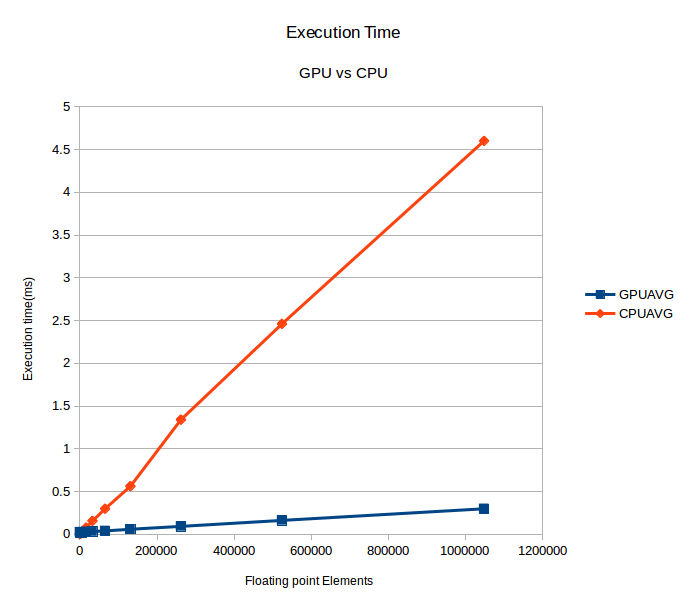
\includegraphics[width=8cm]{execution_time.png}
  \caption{Execution time of CPU vs GPU. Each of the points is the average of 10 consecutive runs.}
  \label{fig:execution_time}
\end{figure}
After some research into the best methods for accessing the memory when performing the summations. It was apparent that banking or memory collisions is a real problem when dealing with parallel sums. Depending on how you access memory greatly increases the speed of the algorithm. The methods presented showed that there are work efficient algorithms as well as hardware efficient algorithms. Work efficient implies that the algorithm roughly has the same running time as the base algorithm. This means that with the parallel algorithm we don't want to increase the number of operations we perform compared to the sequential alternative. However, being work efficient isn't enough. Because memory access is such a slow operation and when multiple threads can't access the same memory location at the same time. If two threads attempt to access the same memory location one will have to wait while the other performs its computation. This essentially serializes the algorithm the more memory collisions there are. A hardware efficient algorithm then attempts to prevent memory collisions entirely.

The algorithm used prevents banking as well as remaining work efficient. It is a simple algorithm that functions on N's that are a power of 2 such that $N=2^m$.
\subsection{Results}
\begin{figure}
  \centering
  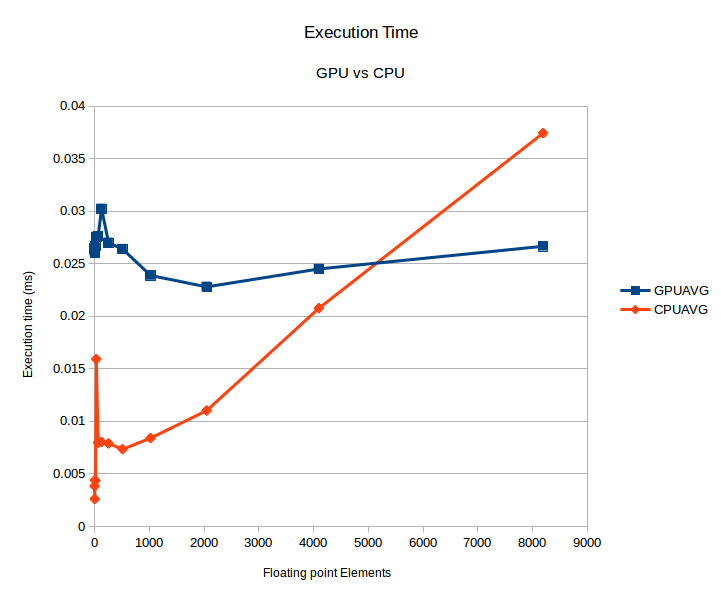
\includegraphics[width=8cm]{execution_time_short.png}
  \caption{Execution time of CPU vs GPU. Each of the points is the average of 10 consecutive runs.}
  \label{fig:execution_short}
\end{figure}
\begin{figure}
  \centering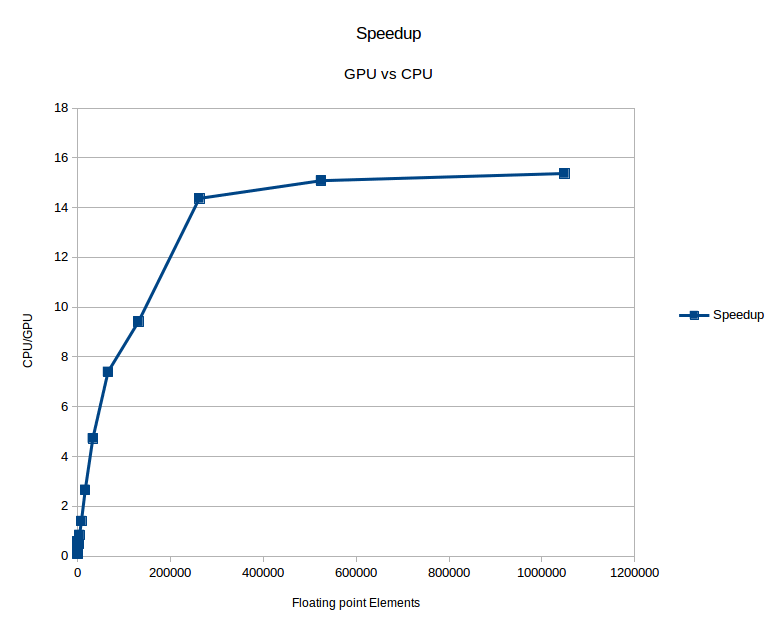
\includegraphics[width=8cm]{speedup.png}
  \caption{Speedup: CPU vs. GPU}
  \label{fig:speedup}
\end{figure}

Performing recursive calls to the GPU isn't always the best and in many cases the fastest method would be to do the initial summation on the GPU followed by a sequential finish of the remaining output sums. The best method is dependent on the size of N(The number of elements in the array). As N becomes large the GPU's parallelization takes effect and drastic speedup are seen. Figure~\ref{fig:execution_short} shows how at small values of N the CPU outperforms the GPU. Considering the effects of I/O with the GPU the use of the GPU after the initial iteration of summation seems less beneficial over the CPU.

Overall the GPU outperforms the CPU when N is large and peaks at around a 15x performance increase over the CPU as seen in figure~\ref{fig:speedup}.


\end{document}

